In de opstelling is er een server gebruikt waaraan alle clienten zich aansluiten via een socket protocol. Met een knop op de pagina worden alle klokken gesynchroniseerd met de server door het tijdsverschil en de vertraging (ping) tussen de laatste twee te berekenen.
Het tijdsverschil wordt namelijk 10 keer herberekend om daar uit mogelijke verbindingsfluctuaties uit te kunnen filteren (meer hierover in sectie [IN TE VULLEN]).

\begin{figure}[h]
\centering
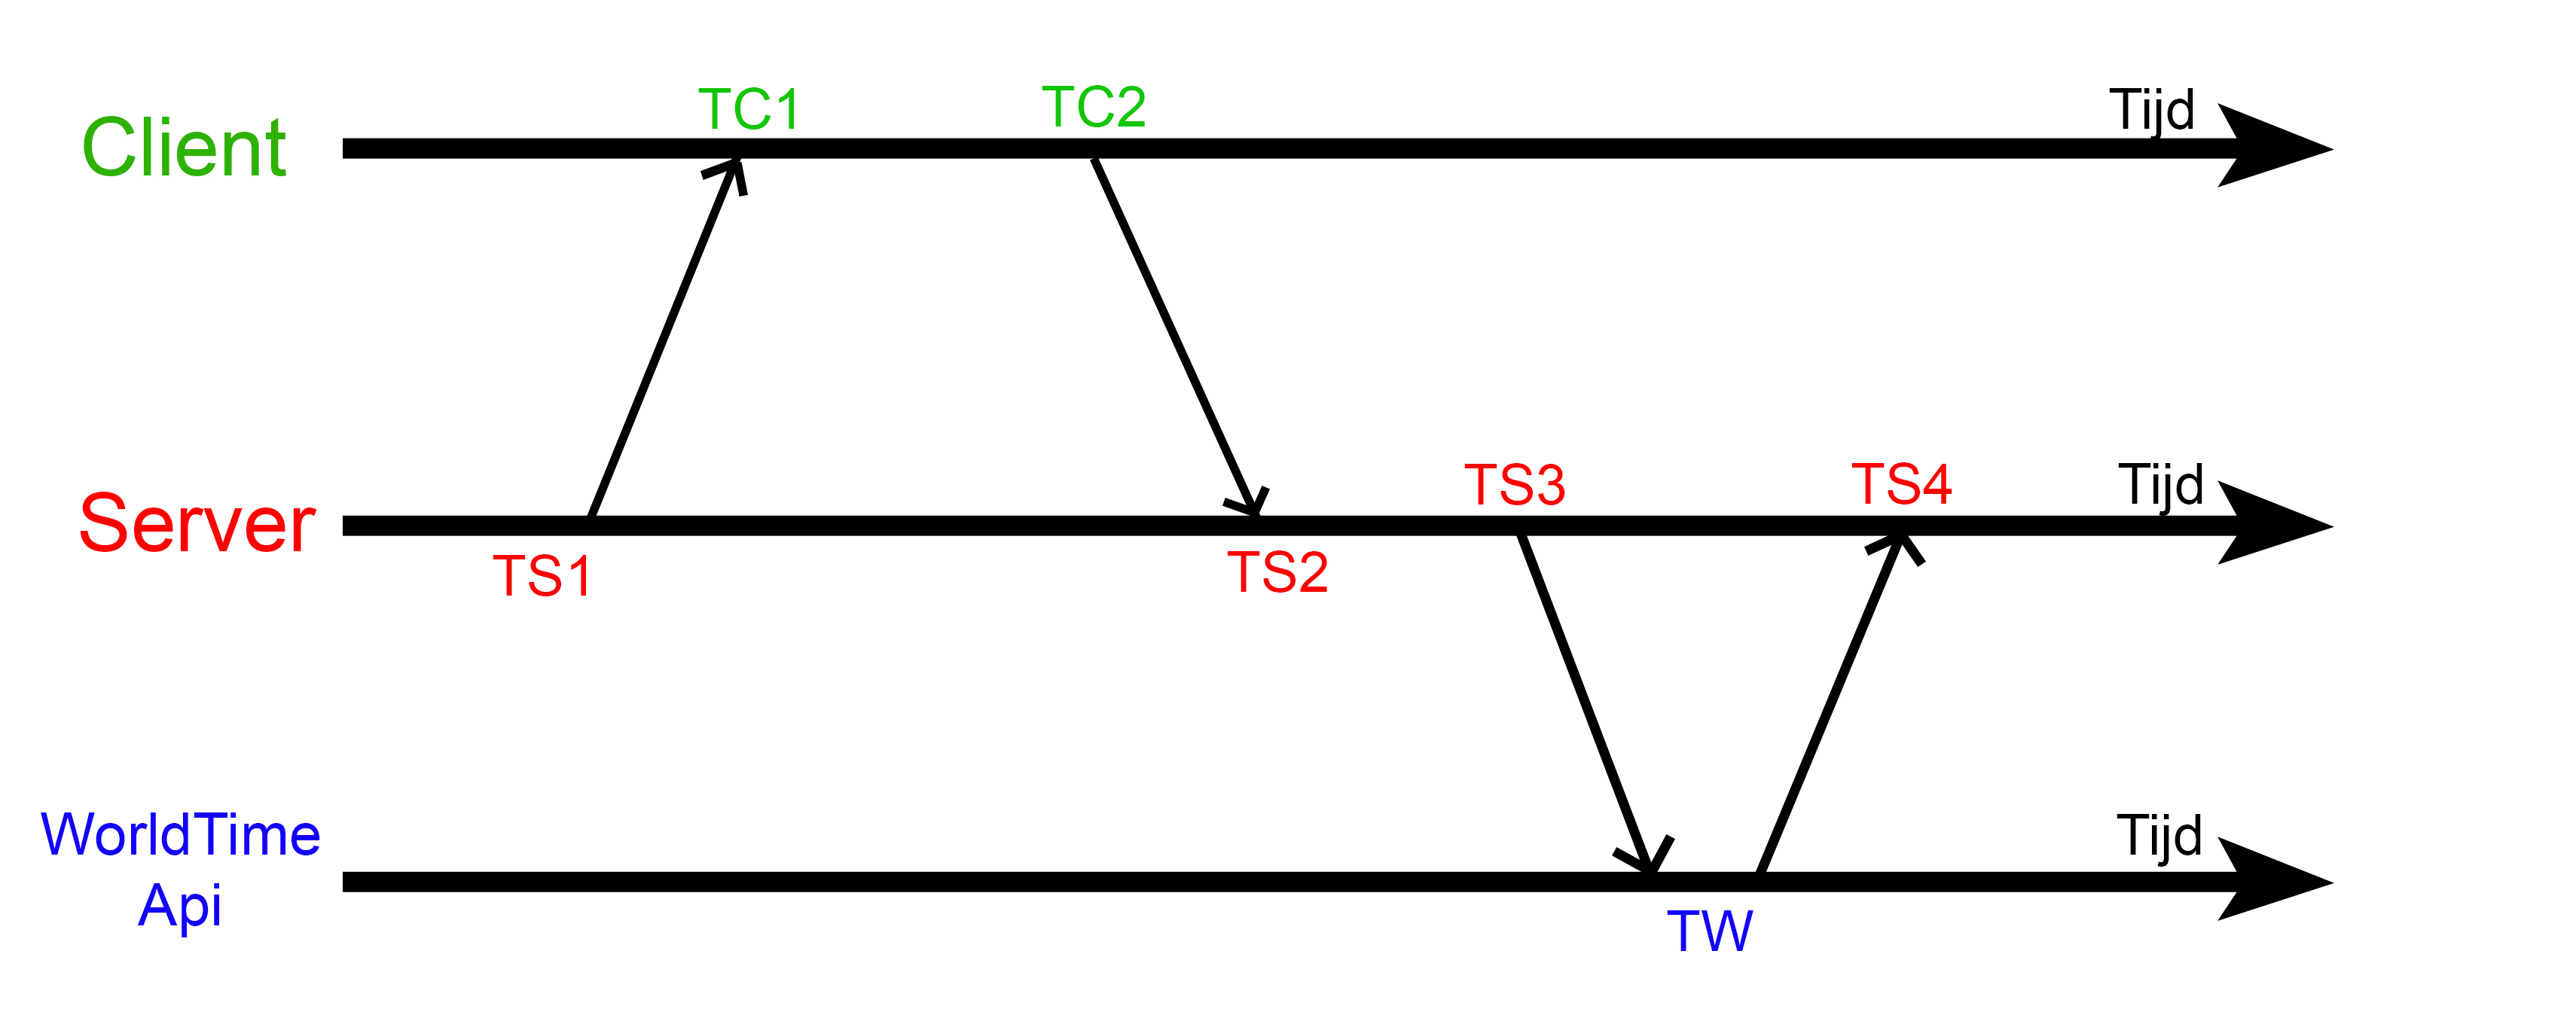
\includegraphics[scale=0.4]{img/server-client-sync.jpg}
\caption{NTP Protocol} \label{serv-client}
\end{figure}

Voor de synchronisatie is het NTP protocol geïmplementeerd. 
Het schema van het NTP protocol is te vinden in figuur \ref{serv-client}. TSx en TCx zijn de tijden gemeten door de server en de client.
Het tijdsverschil wordt gemeten door.
\newline
\[ timeDiff = \frac{(TC1 - TS1) + (TS2 - TC2)}{2}  \]

De vetraging voor de server om een bericht te verzenden en terug te ontvangen is:

\[ ping  = (TS2 - TS2) - (TC2 - TC1) \]


Hiermee is het makkelijk de server tijd te berekenen door de vergelijking:

\[ timeServer = timeClient - timeDiff \]

Om vervolgens de tijdsverschil tussen de server en de wereld tijd te berekenen is er gebruikt gemaakt van een externe api van worldtimeapi.org. Het tijdsverschil is als volgt berekend:

\[ serverWorldOffset = (TW - TS4) + \frac{TS4 - TS3}{2} \]

Uiteindelijk is de volgende informatie opgeslagen:

\begin{itemize}
  \item lijst van ping tussen client en server
  \item tijdsverschil tussen client en server tijd
  \item tijdsverschil server en wereld tijd
  \item tijdsverschil client en wereld tijd
\end{itemize}




